\section{Preprocessing dei Dati}
Il preprocessing dei dati è una fase critica per garantire la qualità e l'efficacia dei modelli di summarization, infatti è fondamentale pulire e filtrare i dati in modo accurato.\\
Sul dataset, per l'appunto, sono stati eseguiti diversi passaggi di pulizia e filtraggio dei dati per garantire qualità e coerenza del modello durante l'addestramento.\\
Vediamo di seguito gli step effettutati durante questa fase:
\subsection{Pulizia del Testo}
Sono stati applicati i seguenti step di preprocessing:

\begin{enumerate}
    \item \textbf{Conversione del testo in minuscolo}
    \begin{itemize}
        \item Questa conversione garantisce l'uniformità del testo, evitando che la stessa parola venga considerata diversa solo per la presenza di maiuscole.\\Ad esempio, "Home", "HOME" e "home" vengono trattate come la stessa parola, riducendo la dimensionalità del vocabolario e migliorando l'efficienza dell'addestramento.
    \end{itemize}

    \item \textbf{Rimozione dei tag HTML}
    \begin{itemize}
        \item Le recensioni potrebbero contenere tag HTML residui dal formato web originale. 
        Questi elementi non contribuiscono al significato semantico del testo e potrebbero interferire con l'apprendimento del modello, pertanto vengono rimossi.
    \end{itemize}

    \item \textbf{Espansione delle contrazioni}
    \begin{itemize}
        \item Le contrazioni nella lingua inglese (come "don't", "I'm", "we're") vengono espanse nelle loro forme complete ("do not", "I am", "we are").\\
        Questo processo vuole standardizzare e garantire coerenza in tutto il testo e aiuta il modello a catturare meglio le relazioni semantiche, eliminando variazioni non necessarie della stessa espressione.
    \end{itemize}

    \item \textbf{Rimozione del genitivo sassone ('s)}
    \begin{itemize}
        \item La forma possessiva in inglese non altera sostanzialmente il significato della frase ai fini del riassunto.\\ 
        La sua rimozione semplifica il testo e riduce ulteriormente la dimensione del vocabolario, permettendo al modello di concentrarsi sui concetti principali.
    \end{itemize}

    \item \textbf{Eliminazione del testo tra parentesi}
    \begin{itemize}
        \item Il testo tra parentesi spesso contiene informazioni supplementari che non sono generalmente essenziali per il riassunto.\\ 
        La rimozione aiuta a mantenere il focus sulle informazioni principali della recensione.
    \end{itemize}

    \item \textbf{Rimozione della punteggiatura e caratteri speciali}
    \begin{itemize}
        \item La punteggiatura e i caratteri speciali, pur essendo importanti per la leggibilità umana, possono introdurre rumore nell'addestramento del modello.\\
        La rimozione semplifica il testo mantenendo intatto il contenuto semantico essenziale per la generazione del riassunto.
    \end{itemize}

    \item \textbf{Eliminazione delle stopwords}
    \begin{itemize}
        \item Le stopwords sono parole molto comuni (come "the", "is", "at", "which") che appaiono frequentemente ma portano poco significato semantico.\\
        La loro rimozione riduce significativamente la dimensionalità del problema senza perdere informazioni cruciali per il riassunto, permettendo al modello di concentrarsi sulle parole più significative.
    \end{itemize}

    \item \textbf{Rimozione delle parole troppo corte}
    \begin{itemize}
        \item Le parole molto corte (solitamente di una o due lettere) spesso non contribuiscono al significato del testo.\\
        La loro rimozione aiuta a ridurre ulteriormente il rumore nei dati, mantenendo solo i termini più significativi per l'analisi.
    \end{itemize}
\end{enumerate}

\subsection{Filtraggio dei Dati}
Dopo l'analisi statistica del dataset, sono stati applicati i seguenti vincoli:
\begin{itemize}
    \item Lunghezza massima delle recensioni: 30 parole
    \item Lunghezza massima dei riassunti: 8 parole
\end{itemize}

Questi limiti sono stati determinati attraverso un'analisi statistica della distribuzione delle lunghezze nel dataset, come possiamo vedere nella figura \ref{fig:dataset_length_distribuition}.
\begin{figure}[H]
    \centering
    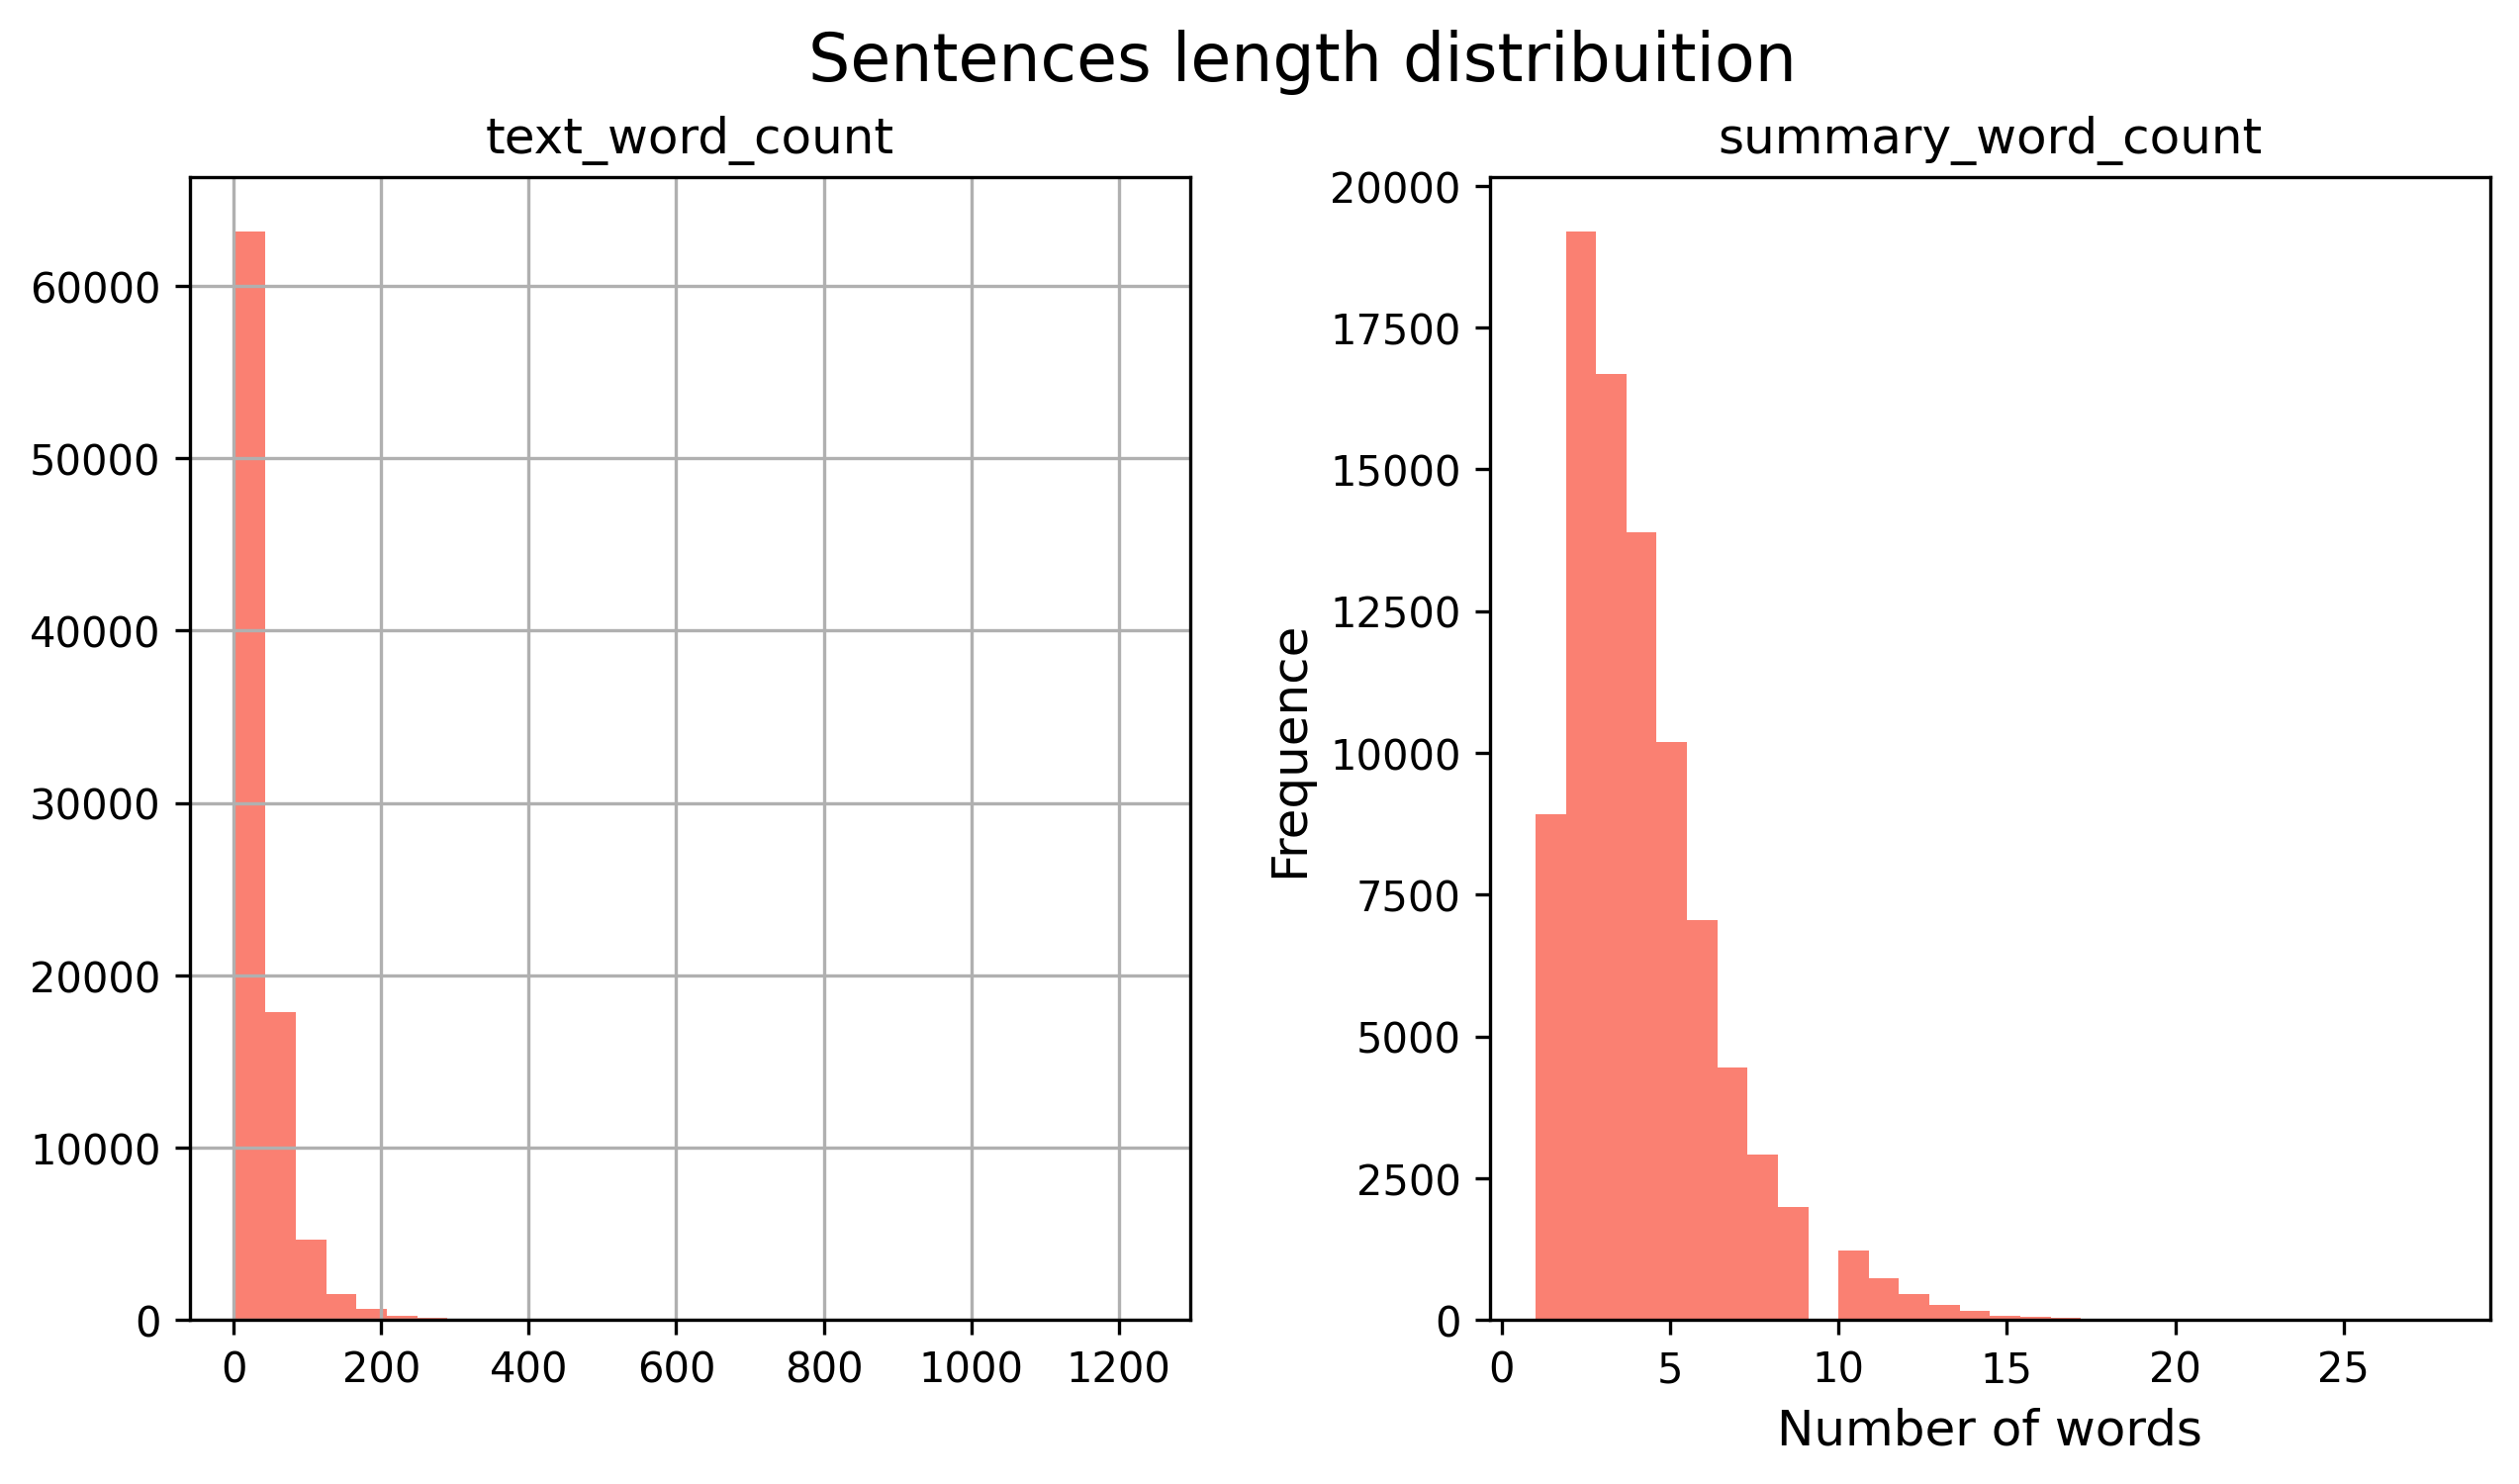
\includegraphics[width=1\textwidth]{media/dataset_length_distribuition.png}
    \caption{A sinistra la distribuzione delle lunghezze delle recensioni, a destra la distribuzione delle lunghezze dei riassunti}
    \label{fig:dataset_length_distribuition}
\end{figure}
Infatti, come si puè notare dai due grafici, la maggior parte delle recensioni e dei riassunti ha lunghezze inferiori ai limiti stabiliti, quindi questi vincoli permettono di mantenere la maggior parte dei dati del dataset.

\subsection{Tokenizzazione e Token Speciali}
Per preparare i dati per i modelli ho aggiunto i token speciali \texttt{"sostok"} e \texttt{"eostok"} per indicare l'inizio e la fine di una sequenza, in modo da facilitare la tokenizzazione e la fase di addestramento.\\
Inoltre, ho effettuato la tokenizzazione separatamente per le recensioni (testo di input) e i riassunti (testo di output) per garantire che il modello possa apprendere correttamente la relazione tra i due.
I due tokenizer servono a creare il vocabolario per le recensioni e per i riassunti, in modo da poter convertire i testi in sequenze di token.
